% !TEX root = ../ds3.tex

%%%%%%%%%%%%%%%%%%%%%%%%%%%%%%%%%%%%%%%%%%%%%%%%%%%%%%%%%%%%%%%%%%%%%%%%%%%%%%%
%%%%%%%%%%%%%%%%%%%%%%%%%%%%%%%%%%%%%%%%%%%%%%%%%%%%%%%%%%%%%%%%%%%%%%%%%%%%%%%
\section{Coordinate descent}
%%%%%%%%%%%%%%%%%%%%%%%%%%%%%%%%%%%%%%%%%%%%%%%%%%%%%%%%%%%%%%%%%%%%%%%%%%%%%%%
%%%%%%%%%%%%%%%%%%%%%%%%%%%%%%%%%%%%%%%%%%%%%%%%%%%%%%%%%%%%%%%%%%%%%%%%%%%%%%%


%%%%%%%%%%%%%%%%%%%%%%%%%%%%%%%%%%%%%%%%%%%%%%%%%%%%%%%%%%%%%%%%%%%%%%%%%%%%%%%
\begin{frame}{Exact Coordinate Descent: idea}

    Goal:
    \begin{align*}
        \min_{w \in \mathbb{R}^p} f(w_1, \dots, w_p)
    \end{align*}
    %
    \pause
    %
    Idea: solve \alert{smaller} and \alert{simpler subproblems}
    %
    \pause

    Algorithm:
    \begin{equation*}
        \begin{aligned}
        \text{for iter}
            & = 1, \dots
            \\
            \text{for }
            & j = 1, \dots, p \quad \text{(cyclic rule)}
            \\
                &
                w_{j}
                \leftarrow
                \argmin_{z \in \mathbb{R}}
                f(w_1, \ldots, w_{j-1}, z, w_{j+1}, \ldots, w_p)
         \end{aligned}
    \end{equation*}
    %
    \pause
    %
    Remarks
    \begin{itemize}
        \item The order of cycle through coordinates is arbitrary, can use any
    permutation of ${1, 2, \dots, n}$
        \item We just have to solve 1D optimization problems but a lot of them...
    \end{itemize}
\end{frame}
%%%%%%%%%%%%%%%%%%%%%%%%%%%%%%%%%%%%%%%%%%%%%%%%%%%%%%%%%%%%%%%%%%%%%%%%%%%%%%%

%%%%%%%%%%%%%%%%%%%%%%%%%%%%%%%%%%%%%%%%%%%%%%%%%%%%%%%%%%%%%%%%%%%%%%%%%%%%%%%
\begin{frame}{Example of CD}
    \centering
    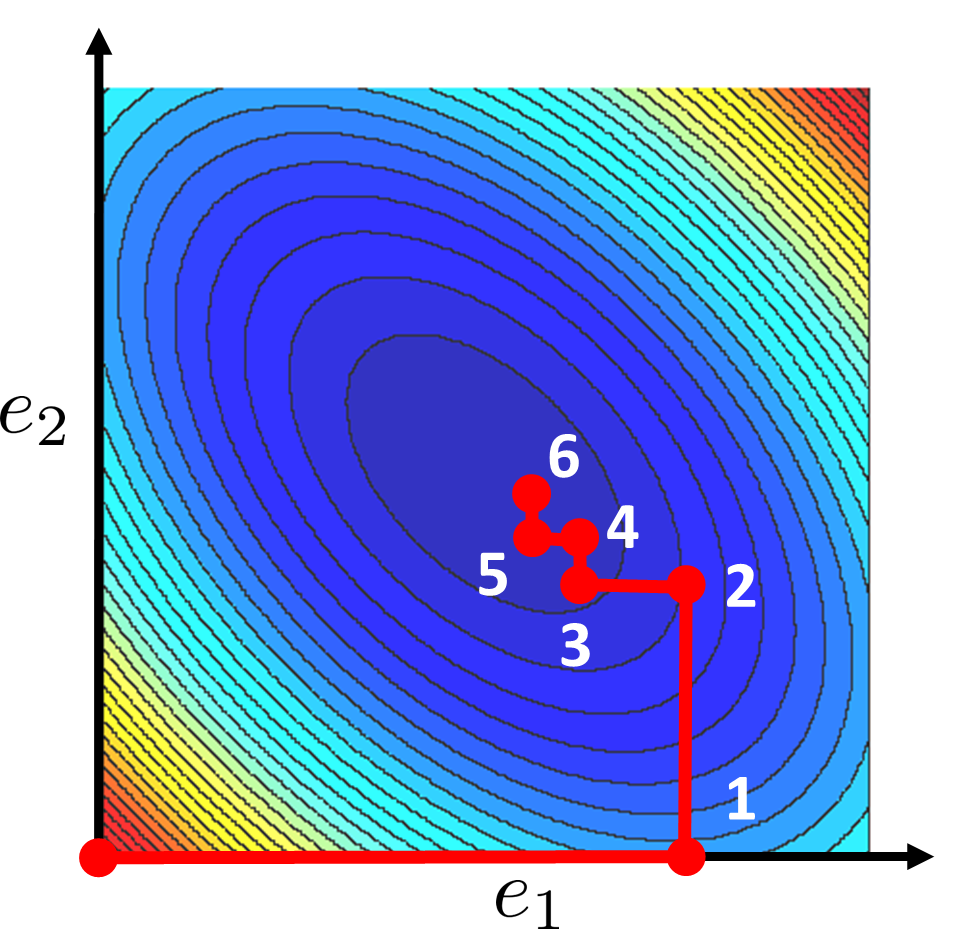
\includegraphics[width=17em]{exampleCD}

    Coordinate descent on a 2D problem
\end{frame}
%%%%%%%%%%%%%%%%%%%%%%%%%%%%%%%%%%%%%%%%%%%%%%%%%%%%%%%%%%%%%%%%%%%%%%%%%%%%%%%

%%%%%%%%%%%%%%%%%%%%%%%%%%%%%%%%%%%%%%%%%%%%%%%%%%%%%%%%%%%%%%%%%%%%%%%%%%%%%%%
\begin{frame}{Exercise: linear regression}
    Derive the exact coordinate descent algorithm for
    \begin{align*}
        f(x)= \frac{1}{2} \|y - A x\|^2
        \enspace ,
    \end{align*}
    where $y \in \bbR^p$, $A \in \bbR^{n \times p}$ is the design matrix.

    \medskip
    \pause

    \textcolor{blue}{TODO correction}

\end{frame}
%%%%%%%%%%%%%%%%%%%%%%%%%%%%%%%%%%%%%%%%%%%%%%%%%%%%%%%%%%%%%%%%%%%%%%%%%%%%%%%

%%%%%%%%%%%%%%%%%%%%%%%%%%%%%%%%%%%%%%%%%%%%%%%%%%%%%%%%%%%%%%%%%%%%%%%%%%%%%%%
\begin{frame}{Coordinate Gradient Descent: algorithm}
    %
    \begin{itemize}
        \item Exact minimization can be expensive
        \item \alert{Idea:} do a \alert{local gradient step} instead of exact minimization
    \end{itemize}
\begin{minipage}{0.49 \textwidth}
    \begin{algorithm}[H]
        \SetKwInOut{Input}{input}
        \SetKwInOut{Init}{init}
        \SetKwInOut{Parameter}{param}
        \caption{CD}
        \Init{ $w = 0_{p}$, $L_1$, \dots, $L_p$}
            \For{$\mathrm{iter} =1,\dots,$}
                {
                \For{$j = 1, \dots, p$}
                    {
                    \tcp{Update only one coef.}

                    $w_j \leftarrow w_j - \frac{1}{L_j} \nabla_j f (w)$
                    }
                }
    \Return{$w$}
    \end{algorithm}
\end{minipage}
%
\begin{minipage}{0.49 \textwidth}
    \begin{algorithm}[H]
        \SetKwInOut{Input}{input}
        \SetKwInOut{Init}{init}
        \SetKwInOut{Parameter}{param}
        \caption{GD}
        \Init{ $w = 0_{p}$, $L$}
            \For{$\mathrm{iter} =1,\dots,$}
                {
                    \tcp{Update all the coef.}

                    $w \leftarrow w - \frac{1}{L} \nabla f (w)$
                }
    \Return{$w$}
    \end{algorithm}
\end{minipage}
\end{frame}
%%%%%%%%%%%%%%%%%%%%%%%%%%%%%%%%%%%%%%%%%%%%%%%%%%%%%%%%%%%%%%%%%%%%%%%%%%%%%%%

%%%%%%%%%%%%%%%%%%%%%%%%%%%%%%%%%%%%%%%%%%%%%%%%%%%%%%%%%%%%%%%%%%%%%%%%%%%%%%%
\begin{frame}{Convergence speed of CD \footfullcite{Beck_Tetruashvili13}}
    Assume $f$ is convex; $\nabla f$ is Lipschitz continuous; $\gamma_j = \frac{1}{L_j}$
    \begin{proposition}[Beck and Tetruashvili (2013)]
    \[
    f(w^{k+1}) - f(w^*)
    \leq
    4 L_{\max} (1+n^3 L_{\max}^2 / L_{\min}^2 ) \frac{R^2(w^0)}{k + 8/n}
    \]
    where
    $R^2(w^0)
    =
    \max_{u, v \in \cV} \{ \|u - v\| :
    f(v) \leq f(u) \leq f(w^0)\}$,
    $L_{\max} = \max_i L_i$
    and $L_{\min} = \min_i L_i$.
    \end{proposition}

    \begin{itemize}
        \item \alert{worst} case complexity rates of CD are bad ($n^3$ complexity) because it is possible to construct adversarial examples \footfullcite{Sun_Ye2019}
        \item However \alert{CD performs surprisingly well} on real-world problems (see labs)
    \end{itemize}
\end{frame}
%%%%%%%%%%%%%%%%%%%%%%%%%%%%%%%%%%%%%%%%%%%%%%%%%%%%%%%%%%%%%%%%%%%%%%%%%%%%%%%


%%%%%%%%%%%%%%%%%%%%%%%%%%%%%%%%%%%%%%%%%%%%%%%%%%%%%%%%%%%%%%%%%%%%%%%%%%%%%%%
\begin{frame}{Exercise: lab4}
    Your turn! Code an $\ell_2$ regularized logistic regression with bias

    \vspace{2em}

    Reminder! All the solutions are in the solutions folder
\end{frame}
%%%%%%%%%%%%%%%%%%%%%%%%%%%%%%%%%%%%%%%%%%%%%%%%%%%%%%%%%%%%%%%%%%%%%%%%%%%%%%%
